% ============================================================================
% DRAFT — Environmental Provisions in Chinese PTAs and Export Composition
% First full draft, 2026-07-06. Compile on Overleaf (pdflatex).
% Figures: copy New/Output/TripleDiff/Diagnostics/*.png into ./figures/
% ============================================================================
\documentclass[12pt]{article}
\usepackage[T1]{fontenc}
\usepackage[utf8]{inputenc}
\usepackage{amsmath, amssymb}
\usepackage{booktabs}
\usepackage{graphicx}
\usepackage{geometry}
\geometry{margin=2.5cm}
\usepackage{setspace}
\onehalfspacing
\usepackage[hidelinks]{hyperref}
\usepackage{threeparttable}
\usepackage[round]{natbib}

\newcommand{\sym}[1]{\rlap{$^{#1}$}}

\title{Do Environmental Provisions in Trade Agreements\\ Reshape Export Composition?\\
\large Evidence from the Universe of Chinese Customs Transactions, 2000--2015\thanks{%
First draft. Comments welcome. All remaining errors are my own.}}
\author{Edoardo Vitella\\ \small University of Trento \& Free University of Bozen}
\date{July 2026 --- \textbf{preliminary draft}}

\begin{document}
\maketitle

\begin{abstract}
\noindent Environmental provisions (EPs) are now ubiquitous in preferential trade agreements
(PTAs), yet evidence on their trade effects remains scarce and is based on aggregate data.
I study whether the EPs contained in the PTAs signed by China between 2000 and 2015 changed
the \emph{composition} of Chinese exports --- shifting firms' export baskets toward
environmental (green) goods and away from pollution-intensive (dirty) goods --- using
transaction-level customs data covering 45.8 million firm--product--destination--year
observations. Identification exploits a triple-difference design: within a given
firm--destination--year, I compare green and dirty products to neutral ones as EP depth
varies across destinations and over time, absorbing the confounding effect of the agreement
itself through firm--destination--year fixed effects. I find a precisely estimated null on
both margins. The green interaction is stable across five estimation designs (full panel,
collapsed panel, and three control-group subsamples), and survives wild cluster bootstrap
and permutation inference. An initially suggestive negative effect on dirty exports does not
survive robust inference: it is driven by a single destination (South Korea) and its
bootstrap p-value is 0.18. Provision-level heterogeneity is not separately identifiable
because Chinese agreements bundle provisions (the two World Bank sub-indices with a direct
trade mechanism are perfectly collinear in-sample). The results contrast with
\citet{brandi2020} and \citet{abman2024}, and suggest that the largely cooperation-based
environmental content of Chinese PTAs in this period had no measurable effect on what China
sells abroad.\\[4pt]
\textbf{Keywords:} trade agreements, environmental provisions, export composition, China.\\
\textbf{JEL:} F13, F14, F18, Q56.
\end{abstract}

\newpage

% ============================================================================
\section{Introduction}
% ============================================================================

Nearly every trade agreement signed in the last two decades contains environmental
language. The TREND database \citep{morin2018} codes roughly 300 distinct types of
environmental provisions (EPs) across more than 700 preferential trade agreements (PTAs),
and the depth of this content has grown steadily. Whether these provisions have real
effects --- on trade flows or on environmental outcomes --- is a question that the
authoritative survey of the trade--environment literature flags as open
\citep{copeland2022}. Two recent papers provide the sharpest evidence to date.
\citet{brandi2020} combine TREND with aggregate bilateral trade flows and find that
trade-restrictive EPs reduce the dirty share, and liberal EPs raise the green share, of
developing-country exports. \citet{abman2024} show that forest- and biodiversity-specific
provisions fully offset the deforestation that otherwise follows entry into force of a
regional trade agreement.

This paper brings the question to the world's largest exporter with the most granular data
available: the universe of Chinese customs transactions, observed at the
firm--product(HS6)--destination--year level (49.2 million observations, roughly 462{,}000
exporting firms). Between 2000 and 2015 China signed around 14 PTAs --- covering 25
destination economies --- whose environmental content ranges from essentially none (the
Bangkok Agreement) to substantial chapters (New Zealand 2008, Switzerland 2014, Korea
2015). I ask whether deeper environmental content shifted the \emph{composition} of
Chinese exports toward green goods and away from dirty goods, relative to neutral
products, within the same firm, destination, and year.

The focus on composition, rather than on export volumes, is dictated by identification.
EP depth in Chinese agreements varies at the destination--year level, enters in force
together with the agreement itself, and afterwards almost never changes (only three
destinations exhibit within-country variation). Any level effect of EP depth on trade is
therefore observationally equivalent to the effect of the agreement, and of agreement
depth in general --- a collinearity that no fixed-effects structure can undo. I document
this formally with a saturation ladder: coefficients on EP depth shrink monotonically to
a precise zero as fixed effects absorb the level of the trade relationship, the signature
of selection into agreements rather than of a causal effect
\citep{bertrand2004, abadie2023}. The composition question, by contrast, is identified:
within a firm--destination--year cell, the agreement affects green, dirty, and neutral
products symmetrically, so their \emph{differential} response to EP depth isolates the
environmental content. The design follows the logic of the classic
industry-$\times$-country interaction of \citet{rajan1998}, and mirrors the ``content
conditional on agreement'' contrast that \citet{abman2024} identify as the credible
margin.

The answer is a precisely estimated null, on both margins. Five independent estimation
designs --- the full firm-level panel, a product--destination--year collapsed panel, and
three control-group subsamples that probe the stability of the coefficient across
comparison sets --- return an EP$\times$green coefficient between $-0.0009$ and
$-0.0023$ (in log points per provision), never remotely significant, with standard errors
around 0.003--0.006. The dynamic version shows flat differential pre-trends and no break
at entry into force. Inference is conducted at three levels --- destination-clustered
asymptotics, wild cluster bootstrap \citep{cameron2008}, and permutation tests that
reshuffle entire EP profiles across treated destinations \citep{fisher1935,bertrand2004}
--- because only 23 destinations (and effectively 14 agreements) are treated. A
suggestive negative coefficient on EP$\times$dirty (asymptotic $p=0.006$ in the collapsed
panel) illustrates exactly why this discipline matters: its wild-bootstrap p-value is
0.18, the permutation test at the aggregate level flips its sign, the TREND index never
confirms it, and a leave-one-out exercise shows it dies when South Korea --- one of only
three destinations with within-country variation in EP depth --- is excluded. The joint
F-test on all four composition interactions in the full firm-level panel is $p=0.26$ (WB
index) and $p=0.71$ (TREND index).

The null is informative rather than disappointing, for three reasons. First, it is
estimated on the near-universe of transactions of the world's dominant exporter, with
tight confidence intervals: economically meaningful composition effects (say, half the
magnitudes in \citealp{brandi2020}) are firmly rejected. Second, its stability across
control groups is itself the result: an artifact of the comparison set would move as the
comparison set moves. Third, it has a coherent economic reading. Decomposing the indices
reveals that Chinese EPs of the period bundle provisions so tightly that the two World
Bank sub-indices with a direct trade mechanism --- green-goods liberalization and
environmental standards --- are \emph{perfectly} collinear in-sample ($\rho = 1.00$), and
most environmental content is soft cooperation language with no trade mechanism at all.
Where \citet{brandi2020} find effects, they are driven by explicitly trade-restrictive or
trade-liberalizing clauses; the Chinese agreements of 2000--2015 contained little of
either, and the data say their environmental chapters did not move trade.

This paper contributes to three literatures: the trade effects of PTA content
\citep{hofmann2017, dur2014, neri2023, baccini2017}, the trade--environment nexus
\citep{cherniwchan2017, shapiro2021, dechezlepretre2017}, and the effectiveness of
environmental clauses in trade agreements \citep{brandi2020, abman2024, morin2018}.
Methodologically, it offers a template for honest inference when treatment varies across
few clusters \citep{cameron2008, abadie2023} and for control-group stability analysis in
triple-difference designs.

The remainder of the paper proceeds as follows. Section~\ref{sec:background} describes
the agreements and the data. Section~\ref{sec:strategy} presents the empirical strategy.
Section~\ref{sec:results} reports the main results, Section~\ref{sec:robust} the
robustness battery, and Section~\ref{sec:conclusion} concludes.

% ============================================================================
\section{Background and data}\label{sec:background}
% ============================================================================

\subsection{Chinese PTAs and their environmental content}

Between 2000 and 2015, PTAs signed by China and entering into force cover 25 destination
economies. Table~\ref{tab:treatment} lists them. Three features of this treatment
landscape discipline everything that follows. First, the ASEAN agreement (2005) covers
eleven destinations with identical values of every EP index: the effective number of
agreements is roughly 14, not 25. Second, EP content is fixed at signature: only three
destinations (notably South Korea, which moved from the shallow Bangkok Agreement to the
deep 2015 FTA) display within-country variation over time. Third, Hong Kong and Macao
(CEPA, 2003) are entrep\^ot economies whose recorded flows are dominated by re-exports;
they account for half of the export value to treated destinations and are excluded from
the main specification (robustness with inclusion reported below).

\begin{table}[htbp]
\centering
\caption{Treatment map: Chinese PTAs in force, 2000--2015}
\label{tab:treatment}
\small
\begin{threeparttable}
\begin{tabular}{lcl}
\toprule
Agreement (partners) & In force & Notes \\
\midrule
Bangkok Agr./APTA (BGD, IND, KOR, LAO, LKA) & 2002/2005 & minimal EP content \\
ASEAN--China (10 members + Timor-Leste, see note) & 2005 & one agreement, 11 destinations \\
Chile & 2006 & \\
Pakistan & 2007 & \\
New Zealand & 2008 & first substantial env.\ chapter \\
Singapore & 2009 & also ASEAN member \\
Peru & 2010 & \\
Costa Rica & 2011 & \\
Iceland; Switzerland & 2014 & richer environmental content \\
Australia; South Korea & 2015 & Korea: one of 3 within-switchers \\
\midrule
Hong Kong; Macao (CEPA) & 2003 & excluded: entrep\^ot, sui generis \\
\bottomrule
\end{tabular}
\begin{tablenotes}\footnotesize
\item Entry-into-force years as coded in the World Bank Deep Trade Agreements database
and TREND; see text. ``Within-switchers'' are destinations whose EP depth changes after
initial entry. Timor-Leste is coded as an ACFTA party in the source databases although
it is not an ASEAN member; it accounts for 0.02\% of observations and the main
coefficients are unchanged to well beyond the fourth decimal if it is dropped (Online
Appendix diagnostic).
\end{tablenotes}
\end{threeparttable}
\end{table}

EP content is measured with two independent codings: the World Bank Deep Trade
Agreements database \citep{hofmann2017}, from which I build \texttt{WB\_EP\_Depth} (the
count of environmental-law provisions in force with destination $d$ at time $t$) and a
non-environmental \texttt{TotalDepth} control; and TREND \citep{morin2018}, from which I
build \texttt{TREND\_EP\_Count} and sub-indices (green market access, enforcement, hard
vs.\ soft provisions). Using two codings guards against idiosyncrasies of either; as
shown below, they agree.

\subsection{Customs data and product classification}

The trade data are the universe of Chinese export customs transactions 2000--2015,
aggregated to the firm--HS6--destination--year level: 49.2 million observations
(45.8 million once Hong Kong and Macao are dropped), about 462{,}000 firms, roughly
5{,}000 HS6 products and 236 destinations. The outcome is the log of export value; the
panel identifiers used for fixed effects (firm--product--destination,
firm--destination--year, product--year) are precomputed.

\emph{Green} products are the 247 HS6 codes of the OECD Combined List of Environmental
Goods. Because the customs panel uses the HS1996 vintage while the OECD list is native
HS2012, the list was translated to HS1996 (a unique 1:1 concordance exists for all 247
codes; export-value continuity checks at the 2002/2007/2012 revision boundaries confirm
a clean mapping). \emph{Dirty} products are the HS6 codes belonging to the classic
pollution-intensive sectors of \citet{mani1998} and \citet{low1992} --- pulp and paper,
industrial chemicals, petroleum refining, iron and steel, non-ferrous metals (plus
cement in an extended list) --- mapped to HS1996 through the official WITS/UNSD
HS1996--ISIC Rev.3 correspondence: 1{,}139 codes. Seventeen codes appearing in both
lists (e.g.\ insulation materials: produced by dirty industries, used for environmental
purposes) are assigned to the green list, which is product-curated; the two categories
are mutually exclusive. Green products account for 11.5\% of firm-level observations and
dirty products for 7.0\%; the remaining ``neutral'' products form the comparison group.

\begin{table}[htbp]
\centering
\caption{Descriptive statistics}
\label{tab:descriptives}
\small
\begin{threeparttable}
\begin{tabular}{lr}
\toprule
Firm-level panel (excl.\ HK--MO) & \\
\midrule
Observations (firm--HS6--dest--year) & 45{,}781{,}211 \\
Exporting firms & $\approx$ 462{,}000 \\
HS6 products & $\approx$ 5{,}000 \\
Destinations & 236 \\
\quad of which treated (EP depth $>0$) & 23 \\
Effective agreements & $\approx$ 14 \\
Share of observations: green products & 11.5\% \\
Share of observations: dirty products & 7.0\% \\
Share of observations under an EP agreement & 20.3\% \\
\midrule
Collapsed panel (HS6--dest--year) & \\
\midrule
Cells & 3{,}773{,}498 \\
\quad green / dirty cells & 8.4\% / 14.0\% \\
Zero-filled PPML grid (HS6--dest--year) & 8{,}310{,}464 \\
\bottomrule
\end{tabular}
\begin{tablenotes}\footnotesize
\item Hong Kong and Macao excluded (they account for 24.4\% of treated observations and
50.1\% of treated export value). Product classification as described in the text.
\end{tablenotes}
\end{threeparttable}
\end{table}

% ============================================================================
\section{Empirical strategy}\label{sec:strategy}
% ============================================================================

\subsection{Why a level effect is not identifiable}

The natural first specification --- regressing log exports on EP depth with fixed
effects --- is uninformative here, and I document this as a diagnostic rather than as a
result. EP depth varies at the destination--year level and switches on with the
agreement; with $\sim$14 agreements and near-zero within-destination variation,
``environmental depth'' and ``having a (deep) agreement'' cannot be told apart. The
saturation ladder makes the point empirically: moving from sparse
(firm--product--destination + year) to saturated (adding product--time and pair-level
interactive effects) structures, the EP-depth coefficient falls monotonically from small
positive and starred to an exact, precisely estimated zero. The pattern --- significance
that lives only in under-saturated, finely-clustered specifications --- is the classic
signature of selection combined with understated standard errors
\citep{bertrand2004, goodmanbacon2021}.

\subsection{The triple-difference on composition}

The main specification is
\begin{equation}\label{eq:main}
\ln x_{fpdt} \;=\; \beta_1\, EP_{dt}\times g_p \;+\; \beta_2\, EP_{dt}\times b_p
\;+\; \gamma_1\, TD_{dt}\times g_p \;+\; \gamma_2\, TD_{dt}\times b_p
\;+\; \theta_{fpd} \;+\; \theta_{fdt} \;+\; \theta_{pt} \;+\; \varepsilon_{fpdt},
\end{equation}
where $f$ indexes firms, $p$ HS6 products, $d$ destinations, $t$ years; $g_p$ and $b_p$
are the green and dirty indicators, $EP_{dt}$ is environmental depth and $TD_{dt}$
non-environmental agreement depth. The firm--destination--year effects $\theta_{fdt}$
are the key: they absorb everything that varies at the level of the firm's relationship
with a market in a year --- including the agreement itself, market size, demand shocks,
and selection into agreements. Identification comes from comparing green (and dirty)
products to neutral ones \emph{within} the same firm--destination--year, as EP content
varies across destinations and over time; $\theta_{pt}$ absorbs global product-level
shocks (e.g.\ the world solar boom) and $\theta_{fpd}$ the level of specialization.
The $TD$ interactions separate environmental content from general agreement depth, the
same role the DESTA index \citep{dur2014} plays in \citet{brandi2020}. Standard errors
are clustered by destination, the level of treatment variation \citep{abadie2023}.

Two complementary implementations address the computational burden of three
high-dimensional fixed effects on 46 million rows. The full panel is estimated with
iterative singleton removal \citep{correia2017}, which eliminates 24.3 million
uninformative observations. A collapsed panel at the HS6--destination--year level (3.77
million cells; outcome: within-cell mean of log exports; regressions weighted by cell
size; fixed effects $pd+dt+pt$), in the gravity-equation tradition of
\citet{headmayer2014}, replicates the identification argument one-for-one --- $dt$ absorbs
the agreement as $fdt$ does in the full panel --- at a fraction of the cost, and the two
give nearly identical answers, an internal cross-validation of both pipelines.

\subsection{Inference with few treated clusters}

There are 236 destination clusters but only 23 treated ones, and effectively 14
agreements. Asymptotic cluster-robust inference is unreliable in this regime, so every
headline estimate is subjected to three tests: (i) destination-clustered asymptotics;
(ii) wild cluster bootstrap with 9{,}999 replications \citep{cameron2008,
fischer2021} --- computed on Frisch--Waugh-residualized data (fixed effects demeaned
once, not re-estimated at each bootstrap draw), an approximation that treats $pt$ as if
it were nested within the destination cluster, which it is not, while $pd$ and $dt$ are;
demeaned coefficients match the unrestricted \texttt{fixest} estimates exactly --- and
(iii) permutation inference \citep{fisher1935}: entire EP profiles
(depth and timing) are randomly reassigned 1{,}000 times across treated destinations,
asking whether the observed coefficient stands out among placebos --- the sharpest
answer to ``is it really the environmental content, or would any labelling of these
destinations produce this number?''. The dynamic specification is an event study of the
green (dirty) vs.\ neutral differential around entry into force, with never-treated
destinations as controls, endpoint bins declared, and a Sun--Abraham version
\citep{sun2021} run on the destination-level composition gap to address staggered-timing
cohort heterogeneity \citep{goodmanbacon2021, dechaisemartin2020, callaway2021}.

% ============================================================================
\section{Main results}\label{sec:results}
% ============================================================================

\subsection{The green margin: a stable, precise null}

Table~\ref{tab:main} reports the main estimates. In the full firm-level panel the
EP$\times$green coefficient is $-0.0021$ (s.e.\ 0.0034) with the WB index and $-0.0001$
(s.e.\ 0.0010) with TREND; the joint F-test on all four composition interactions is
$p=0.26$ and $p=0.71$ respectively. The collapsed panel returns $-0.0023$ (WB): the wild
cluster bootstrap p-value is 0.88, and the permutation p-value 0.45. To gauge magnitudes:
a one-standard-deviation increase in WB EP depth across treated destination--years
($\approx$ 3 provisions) is associated with at most a 2.7\% decline in green relative
to neutral exports at the lower 95\% confidence bound of the full-panel estimate ---
economically negligible against the effects in \citet{brandi2020}.

\begin{table}[htbp]
\centering
\caption{Triple-difference estimates: EP content and export composition}
\label{tab:main}
\small
\begin{threeparttable}
\begin{tabular}{lcccc}
\toprule
 & \multicolumn{2}{c}{WB EP depth} & \multicolumn{2}{c}{TREND EP count} \\
\cmidrule(lr){2-3}\cmidrule(lr){4-5}
 & $\times$ green & $\times$ dirty & $\times$ green & $\times$ dirty \\
\midrule
\textbf{Full panel} (reghdfe) & $-0.0021$ & $-0.0040$\sym{*} & $-0.0001$ & $-0.0009$ \\
 & (0.0034) & (0.0019) & (0.0010) & (0.0006) \\
\quad asymptotic $p$ & 0.55 & 0.038 & 0.91 & 0.15 \\
\addlinespace
\textbf{Collapsed panel} & $-0.0023$ & $-0.0089$ & $+0.0018$ & $+0.0004$ \\
 & (0.0063) & (0.0032) & (0.0018) & (0.0016) \\
\quad asymptotic $p$ & 0.72 & 0.006 & 0.32 & 0.83 \\
\quad wild cluster bootstrap $p$ & 0.88 & 0.18 & 0.39 & 0.85 \\
\quad permutation $p$ & 0.45 & 0.50$^{\dagger}$ & --- & --- \\
\bottomrule
\end{tabular}
\begin{tablenotes}\footnotesize
\item Full panel: 21{,}519{,}511 obs.\ after iterative singleton removal, FE
$fpd+fdt+pt$, 225 destination clusters; joint F on the four interactions: $p=0.26$ (WB),
$p=0.71$ (TREND). Collapsed panel: 3{,}681{,}023 cells (3{,}773{,}498 before
fixed-effect singleton removal), FE $pd+dt+pt$, weighted, 236 clusters. All specifications include TotalDepth$\times$green/dirty controls. Wild
cluster bootstrap: B=9{,}999 \citep{cameron2008}. Permutation: 1{,}000 reassignments of
entire EP profiles across treated destinations, estimated on a destination--year--product-type
aggregate of the collapsed panel (observed coefficients: $-0.0052$ green, $+0.004$
dirty$^{\dagger}$); p-values are the share of placebo assignments producing a larger
absolute coefficient. $^{\dagger}$sign reverses at this aggregate level. \sym{*} $p<0.05$
(asymptotic only; see text).
\end{tablenotes}
\end{threeparttable}
\end{table}

\subsection{Stability across control groups}

Table~\ref{tab:stability} re-estimates equation~\eqref{eq:main} on subsamples that
progressively tighten the comparison group: non-green products in the same HS4 family
as a green product; destinations retained by a coarsened-exact-matching country match
\citep{iacus2012}; PTA partners only, comparing deep- to shallow-EP agreements (the
within-treated contrast of \citealp{abman2024}); and products in common support.
The green coefficient barely moves --- between $-0.0009$ and $-0.0023$ --- and is never
significant. The stability is the point: a comparison-group artifact would move with the
comparison group.

\begin{table}[htbp]
\centering
\caption{Stability of the EP$\times$green coefficient across estimation designs (WB index)}
\label{tab:stability}
\small
\begin{threeparttable}
\begin{tabular}{lccc}
\toprule
Design & Effective sample & EP$\times$green & $p$ \\
\midrule
Full panel (firm level) & 21.5M & $-0.0021$ & 0.55 \\
Collapsed panel & 3.7M cells & $-0.0023$ & 0.72 \\
C-prod-HS4 (within green HS4 families) & 3.8M & $-0.0009$ & 0.84 \\
CEM-matched destinations & 13.7M & $-0.0022$ & 0.49 \\
Deep vs.\ shallow (PTA partners only) & 5.3M & $-0.0021$ & 0.50 \\
Common support (C-overlap) & 21.5M & $-0.0021$ & 0.55 \\
Full panel, with controls & 19.3M & $-0.0002$ & 0.93 \\
Full panel, excluding ASEAN & 19.2M & $-0.0025$ & 0.42 \\
Full panel, including HK--Macao & 23.6M & $-0.0011$ & 0.73 \\
\bottomrule
\end{tabular}
\begin{tablenotes}\footnotesize
\item Each row estimates equation~\eqref{eq:main} on the indicated subsample;
destination-clustered s.e. CEM match on log GDP p.c., growth, MFN tariff (year 2000).
Deep/shallow split at the median of maximum EP depth (17 deep vs.\ 6 shallow countries
in the estimation sample, which excludes Hong Kong and Macao).
TREND-index analogues (where estimated) give the same picture: full panel $-0.0001$
($p=0.91$), common support $-0.0001$ ($p=0.91$), deep vs.\ shallow $-0.0004$ ($p=0.72$).
Controls: MFN tariff, market concentration (HHI), antidumping indicator.
\end{tablenotes}
\end{threeparttable}
\end{table}

\subsection{Dynamics}

Figure~\ref{fig:es} plots the event study. Differential pre-trends are flat for both
green and dirty products --- the identifying assumption is visible, not assumed --- and
nothing happens at entry into force. The late negative drift for green products (bin
$\geq$+5) is identified only by early cohorts (ASEAN 2005, Chile 2006, Pakistan 2007,
New Zealand 2008) and does not survive the Sun--Abraham estimator applied to the
destination-level composition gap: the aggregated ATT is $-0.044$ ($p=0.24$) for the
green gap and $+0.073$ ($p=0.28$) for the dirty gap --- consistent with cohort
heterogeneity rather than a treatment effect \citep{sun2021}.

\begin{figure}[htbp]
\centering
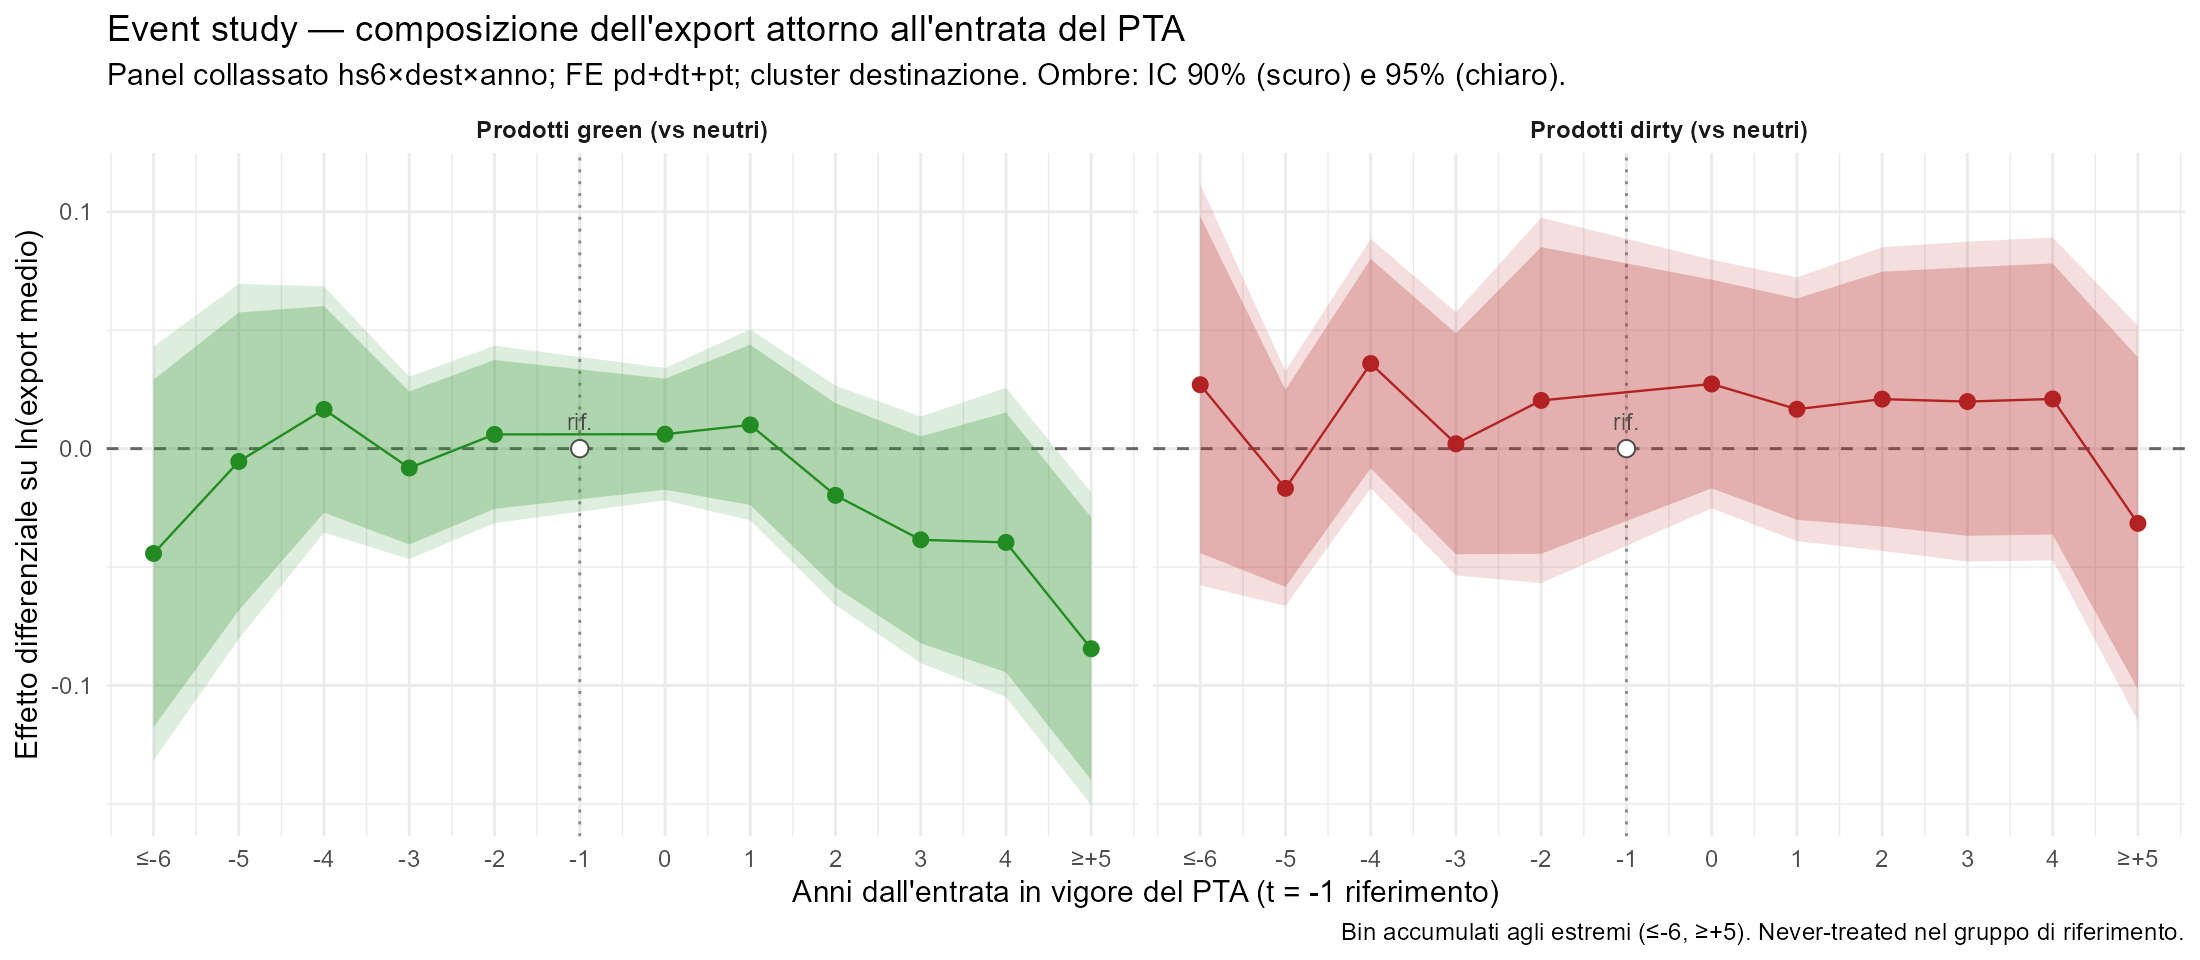
\includegraphics[width=\textwidth]{figures/eventstudy_collapsed_v2.png}
\caption{Event study: green and dirty vs.\ neutral products around PTA entry into
force. Collapsed panel; FE $pd+dt+pt$; destination-clustered 90\% (dark) and 95\%
(light) bands; $t=-1$ is the reference period; endpoint bins accumulate.}
\label{fig:es}
\end{figure}

\subsection{The dirty margin: anatomy of a false positive}\label{sec:dirty}

The asymptotically significant WB$\times$dirty coefficient in the collapsed panel
($-0.0089$, $p=0.006$) deserves its own subsection, because it is a textbook
illustration of few-cluster inference. Three independent tests dismantle it. The wild
cluster bootstrap raises its p-value to 0.18. Permutation inference on the aggregate
destination--year--dirty panel reverses its sign (+0.004, $p=0.50$). And a
leave-one-out exercise across the 23 treated destinations shows the coefficient is
stable ($\approx -0.009$) except when South Korea is dropped, in which case it falls to
$-0.0059$ with $p=0.21$: Korea is one of only three destinations with within-country
variation in EP depth (the 2015 FTA), and carries a disproportionate share of the
identifying variation. The TREND index never shows the effect (bootstrap $p=0.85$). In
the full firm-level panel the coefficient is $-0.0040$ with an asymptotic $p$ of 0.038
--- the same magnitude as in the CEM subsample, and exactly the kind of marginal
asymptotic significance that the collapsed-panel exercise shows evaporating under
robust inference.

% ============================================================================
\section{Robustness and extensions}\label{sec:robust}
% ============================================================================

\subsection{Provision bundling and the limits of heterogeneity analysis}

A natural objection is that the aggregate index dilutes provisions with a trade
mechanism (green-goods liberalization; binding standards) with cooperation language that
has none. The objection is correct in principle --- and unanswerable in this setting,
which is itself a finding. Across the 223 treated country--year observations in the
estimation sample, the two WB sub-indices with a direct mechanism
(\texttt{GreenLiberalization} and \texttt{StandardsNonRegression}) are \emph{perfectly}
collinear ($\rho = 1.000$) --- and the reason is stark: both are non-zero in only three
country--years (Korea from 2015; Switzerland from 2014), always in the same 1:3
proportion. Mechanism-bearing provisions effectively exist in two Chinese agreements of
the period. Their interactions load identically in the regression (identical
t-statistics; coefficients in exact 3:1 ratio). TREND
sub-indices correlate between 0.5 and 0.9 with each other and with the total count.
With $\sim$14 agreements, provision-type heterogeneity is not separately identifiable
--- in sharp contrast with \citet{brandi2020}, whose 680-agreement panel allows it (they
report a maximum VIF of 4.6; here it is unbounded). What can be said: the
mechanism-bearing bundle shows the same pattern as the aggregate index --- green never
responds (green-liberalization $\times$ green: $p=0.90$; TREND green-market-access
$\times$ green: $p=0.38$), while the dirty interaction is marginally negative on
asymptotic p-values ($p=0.04$--$0.07$), the same fragile signal as the aggregate. The
placebo components with no trade mechanism (TREND soft provisions, regulatory-space
clauses) show nothing on either margin ($p \geq 0.27$), which is reassuring: a selection
story would light up precisely there. Enforcement provisions --- dispute-settlement
mechanisms attached to the environmental chapter, which condition whether any of the
above is binding rather than providing a trade mechanism themselves --- are likewise
null on both margins and both codings (WB \texttt{EnforcementDSM} $\times$ green:
$p=0.91$; $\times$ dirty: $p=0.90$; TREND \texttt{EnforcementDSM} $\times$ green:
$p=0.78$; $\times$ dirty: $p=0.71$).

\subsection{Extensive margin}

Log-linear estimates condition on positive flows. If EPs created green trade at the
extensive margin --- new firm--product--destination combinations --- the intensive
estimates would miss it \citep{santossilva2006, larch2025}. On a zero-filled
HS6--destination--year grid (8.3 million cells), PPML estimates of
equation~\eqref{eq:main}'s aggregated analogue confirm the null: EP$\times$green is
$+0.0014$ ($p=0.73$) with the WB index and $+0.0001$ ($p=0.95$) with TREND;
EP$\times$dirty is $-0.021$ ($p=0.16$) and $+0.003$ ($p=0.55$) respectively. There is
no green trade creation at the extensive margin.

\subsection{Within-firm reallocation}

The margin that aggregate data cannot see: does the green \emph{share} of a
multiproduct firm's basket toward a destination respond to EP depth? On the
firm--destination--year panel of green shares (13.3 million observations; FE:
firm--destination and year; destination-clustered s.e.), the coefficient on WB EP
depth is $-0.00014$ ($p=0.37$) and on the TREND count $-0.00006$ ($p=0.044$,
asymptotic). Both are economically negligible: a one-standard-deviation increase in
the TREND count moves the within-firm green share by three hundredths of a percentage
point, with the ``wrong'' sign, and the marginal asymptotic significance is subject to
the same few-clusters caveat as everything else in this setting. Chinese firms did not
rebalance their baskets. This module speaks to the within-plant evidence of
\citet{cherniwchan2017}: where NAFTA tariff cuts changed what plants do, Chinese EP
chapters did not change what exporters sell.

\subsection{Sample robustness}

Table~\ref{tab:robust} collects the full-panel sample variations. Adding controls (MFN
tariff, market concentration, antidumping exposure) moves the green coefficient to an
exact zero ($-0.0002$, $p=0.93$). Excluding the eleven ASEAN destinations --- the block
that dominates the treated count --- leaves it at $-0.0025$ ($p=0.42$). Re-including
Hong Kong and Macao gives $-0.0011$ ($p=0.73$). Restricting to common-support products
gives $-0.0021$ ($p=0.55$). Across every variation the dirty coefficient sits between
$-0.004$ and $-0.0055$ with asymptotic p-values between 0.02 and 0.05 --- persistently
marginal, and, as Section~\ref{sec:dirty} established, not robust to bootstrap,
permutation, or leave-one-out inference.

\begin{table}[htbp]
\centering
\caption{Sample robustness (full firm-level panel, WB index)}
\label{tab:robust}
\small
\begin{threeparttable}
\begin{tabular}{lcccc}
\toprule
Variation & Obs. & EP$\times$green ($p$) & EP$\times$dirty ($p$) \\
\midrule
Baseline & 21.5M & $-0.0021$ (0.55) & $-0.0040$ (0.038) \\
With controls & 19.3M & $-0.0002$ (0.93) & $-0.0055$ (0.022) \\
Excluding ASEAN & 19.2M & $-0.0025$ (0.42) & $-0.0041$ (0.031) \\
Including HK--Macao & 23.6M & $-0.0011$ (0.73) & $-0.0040$ (0.050) \\
Common support & 21.5M & $-0.0021$ (0.55) & $-0.0040$ (0.038) \\
\midrule
PPML, zero-filled grid & 8.3M cells & $+0.0014$ (0.73) & $-0.021$ (0.16) \\
Within-firm green share & 13.3M & \multicolumn{2}{c}{$-0.00014$ (0.37)} \\
\bottomrule
\end{tabular}
\begin{tablenotes}\footnotesize
\item Asymptotic destination-clustered p-values in parentheses; the dirty column's
marginal significance does not survive wild cluster bootstrap, permutation, or
leave-one-out inference (Section~\ref{sec:dirty}). Controls: ln(1+MFN tariff), ln HHI,
antidumping indicator.
\end{tablenotes}
\end{threeparttable}
\end{table}

A remaining caveat: the tariff control is the MFN rate, not the bilateral preferential
rate (the WITS-TRAINS API was unavailable at the time of writing); this is mitigated by
the fact that tariff liberalization varies at the destination--year level and is
absorbed by $\theta_{fdt}$, and at the product level by the $TD$ interactions.

% ============================================================================
\section{Conclusion}\label{sec:conclusion}
% ============================================================================

Using the universe of Chinese customs transactions and two independent codings of the
environmental content of China's trade agreements, this paper finds that environmental
provisions did not change what China exports: not the green share, not the dirty share,
not the extensive margin, not the within-firm basket. The null is precise, stable
across estimation designs and sample variations, and survives an inference battery
designed for the few-treated-clusters regime that characterizes this --- and most ---
PTA settings.

The reading is not that environmental provisions never matter: \citet{abman2024} show
they can, on environmental outcomes, when they are specific and enforceable. The reading
is that the environmental chapters China signed in 2000--2015 --- thin, bundled, and
dominated by cooperation language --- had no trade bite. For the policy debate on
greening trade agreements, the distinction matters: content design, not chapter
presence, is what could move flows. For the empirical literature, the paper adds a
cautionary methodological tale: with treatment varying across a dozen agreements,
asymptotically significant composition effects appear and dissolve under honest
inference; the discipline of bootstrap, permutation, and leave-one-out should be
standard equipment.

% ============================================================================
\begin{thebibliography}{99}
% ============================================================================

\bibitem[Abadie et al.(2023)]{abadie2023}
Abadie, A., Athey, S., Imbens, G.~W., \& Wooldridge, J.~M. (2023).
When should you adjust standard errors for clustering?
\emph{Quarterly Journal of Economics}, 138(1), 1--35.

\bibitem[Abman et al.(2024)]{abman2024}
Abman, R., Lundberg, C., \& Ruta, M. (2024).
The effectiveness of environmental provisions in regional trade agreements.
\emph{Journal of the European Economic Association}, 22(6), 2507--2548.

\bibitem[Baccini et al.(2017)]{baccini2017}
Baccini, L., Pinto, P.~M., \& Weymouth, S. (2017).
The distributional consequences of preferential trade liberalization: firm-level evidence.
\emph{International Organization}, 71(2), 373--395.

\bibitem[Bertrand et al.(2004)]{bertrand2004}
Bertrand, M., Duflo, E., \& Mullainathan, S. (2004).
How much should we trust differences-in-differences estimates?
\emph{Quarterly Journal of Economics}, 119(1), 249--275.

\bibitem[Brandi et al.(2020)]{brandi2020}
Brandi, C., Schwab, J., Berger, A., \& Morin, J.-F. (2020).
Do environmental provisions in trade agreements make exports from developing countries greener?
\emph{World Development}, 129, 104899.

\bibitem[Callaway \& Sant'Anna(2021)]{callaway2021}
Callaway, B., \& Sant'Anna, P.~H.~C. (2021).
Difference-in-differences with multiple time periods.
\emph{Journal of Econometrics}, 225(2), 200--230.

\bibitem[Cameron et al.(2008)]{cameron2008}
Cameron, A.~C., Gelbach, J.~B., \& Miller, D.~L. (2008).
Bootstrap-based improvements for inference with clustered errors.
\emph{Review of Economics and Statistics}, 90(3), 414--427.

\bibitem[Cherniwchan(2017)]{cherniwchan2017}
Cherniwchan, J. (2017).
Trade liberalization and the environment: evidence from NAFTA and U.S. manufacturing.
\emph{Journal of International Economics}, 105, 130--149.

\bibitem[Copeland et al.(2022)]{copeland2022}
Copeland, B.~R., Shapiro, J.~S., \& Taylor, M.~S. (2022).
Globalization and the environment.
In \emph{Handbook of International Economics} (Vol.~5, pp.~61--146). Elsevier.

\bibitem[Correia(2017)]{correia2017}
Correia, S. (2017).
Linear models with high-dimensional fixed effects: an efficient and feasible estimator.
Working paper.

\bibitem[de Chaisemartin \& D'Haultf\oe uille(2020)]{dechaisemartin2020}
de Chaisemartin, C., \& D'Haultf\oe uille, X. (2020).
Two-way fixed effects estimators with heterogeneous treatment effects.
\emph{American Economic Review}, 110(9), 2964--2996.

\bibitem[Dechezlepr\^etre \& Sato(2017)]{dechezlepretre2017}
Dechezlepr\^etre, A., \& Sato, M. (2017).
The impacts of environmental regulations on competitiveness.
\emph{Review of Environmental Economics and Policy}, 11(2), 183--206.

\bibitem[D\"ur et al.(2014)]{dur2014}
D\"ur, A., Baccini, L., \& Elsig, M. (2014).
The design of international trade agreements: introducing a new dataset.
\emph{Review of International Organizations}, 9(3), 353--375.

\bibitem[Fischer \& Roodman(2021)]{fischer2021}
Fischer, A., \& Roodman, D. (2021).
fwildclusterboot: fast wild cluster bootstrap inference for linear regression models.
R package.

\bibitem[Fisher(1935)]{fisher1935}
Fisher, R.~A. (1935).
\emph{The Design of Experiments}. Oliver \& Boyd.

\bibitem[Goodman-Bacon(2021)]{goodmanbacon2021}
Goodman-Bacon, A. (2021).
Difference-in-differences with variation in treatment timing.
\emph{Journal of Econometrics}, 225(2), 254--277.

\bibitem[Head \& Mayer(2014)]{headmayer2014}
Head, K., \& Mayer, T. (2014).
Gravity equations: workhorse, toolkit, and cookbook.
In \emph{Handbook of International Economics} (Vol.~4, pp.~131--195). Elsevier.

\bibitem[Hofmann et al.(2017)]{hofmann2017}
Hofmann, C., Osnago, A., \& Ruta, M. (2017).
Horizontal depth: a new database on the content of preferential trade agreements.
\emph{World Bank Policy Research Working Paper}, 7981.

\bibitem[Iacus et al.(2012)]{iacus2012}
Iacus, S.~M., King, G., \& Porro, G. (2012).
Causal inference without balance checking: coarsened exact matching.
\emph{Political Analysis}, 20(1), 1--24.

\bibitem[Larch et al.(2025)]{larch2025}
Larch, M., Shikher, S., \& Yotov, Y.~V. (2025).
Estimating gravity equations: theory implications, econometric developments, and
practical recommendations.
\emph{Review of International Economics}, 33(5), 1066--1092.

\bibitem[Low \& Yeats(1992)]{low1992}
Low, P., \& Yeats, A. (1992).
Do ``dirty'' industries migrate?
In P.~Low (ed.), \emph{International Trade and the Environment},
World Bank Discussion Paper 159.

\bibitem[Mani \& Wheeler(1998)]{mani1998}
Mani, M., \& Wheeler, D. (1998).
In search of pollution havens? Dirty industry in the world economy, 1960--1995.
\emph{Journal of Environment \& Development}, 7(3), 215--247.

\bibitem[Morin et al.(2018)]{morin2018}
Morin, J.-F., D\"ur, A., \& Lechner, L. (2018).
Mapping the trade and environment nexus: insights from a new dataset.
\emph{Global Environmental Politics}, 18(1), 122--139.

\bibitem[Neri-Lain\'e et al.(2023)]{neri2023}
Neri-Lain\'e, M., Orefice, G., \& Ruta, M. (2023).
Deep trade agreements and heterogeneous firms' exports.
\emph{CESifo Working Paper}, 10436.

\bibitem[Rajan \& Zingales(1998)]{rajan1998}
Rajan, R.~G., \& Zingales, L. (1998).
Financial dependence and growth.
\emph{American Economic Review}, 88(3), 559--586.

\bibitem[Santos Silva \& Tenreyro(2006)]{santossilva2006}
Santos Silva, J.~M.~C., \& Tenreyro, S. (2006).
The log of gravity.
\emph{Review of Economics and Statistics}, 88(4), 641--658.

\bibitem[Shapiro(2021)]{shapiro2021}
Shapiro, J.~S. (2021).
The environmental bias of trade policy.
\emph{Quarterly Journal of Economics}, 136(2), 831--886.

\bibitem[Sun \& Abraham(2021)]{sun2021}
Sun, L., \& Abraham, S. (2021).
Estimating dynamic treatment effects in event studies with heterogeneous treatment effects.
\emph{Journal of Econometrics}, 225(2), 175--199.

\end{thebibliography}
\end{document}
